%%%%%%%%%%%%%%%%%%%%%%%%%%%%%%%%%%%
\chapter{Comunidades}\label{comunidades}
%%%%%%%%%%%%%%%%%%%%%%%%%%%%%%%%%%%
% \redcomment{Revisar tradução e texto}
% Focar no Paper
Neste capítulo discutimos sobre as comunidades científicas que utilizamos em nossas análises e, em seguida, apresentamos
uma definição para identificação do que chamamos de núcleo das comunidades.

%%%%%%%%%%%%%%%%%%%%%%%%%%%%%%%%%%%
\section{Comunidades Científicas}
%%%%%%%%%%%%%%%%%%%%%%%%%%%%%%%%%%%

Dada uma rede social, uma comunidade pode ser compreendida como um grupo denso de nodos dessa rede que possuem mais arestas 
interligando-os entre si, do que arestas interligando-os ao restante da rede. Existem múltiplas definições e estratégias 
para identificar comunidades e elas variam de acordo com o contexto~\citep{Kleinberg2008,Leskovec2010}. No nosso contexto, 
uma comunidade científica pode ser definida em termos de uma grande e consolidada conferência científica capaz de reunir 
pesquisadores que trabalham em uma mesma área de pesquisa ao longo de vários anos.
% The notion of community can be understood as a dense group of nodes in a network, with more edges inside than edges linking the rest of the network.  There are multiple definitions
% and strategies of identifying communities and they vary according to the context~\cite{Kleinberg@cacm2008,Leskovec@www2010}. In our context, a scientific community is defined in terms of a large and well established
% scientific conference able to aggregate researchers working in similar research topics along a considerable number of years. 
 
A fim de construir um conjunto de comunidades científicas, coletamos dados da DBLP\footnote{http://dblp.uni-trier.de/}~\citep{Ley2009}, 
uma biblioteca digital que contém mais de 2,1 milhões de publicações de 1,2 milhões de autores e que provê informações 
bibliográficas dos principais anais de conferências e periódicos da área de Ciência da Computação. A DBLP disponibiliza 
todo o seu conjunto de dados no formato XML (\textit{eXtensible Markup Language}), o que facilita a obtenção dos dados e a 
construção de comunidades científicas inteiras.
% In order to construct a set of scientific communities, we have gathered data from DBLP\footnote{http://dblp.uni-trier.de/}~\cite{Ley:2009}, a digital library containing more
% than 2.1 million publications from 1.2 million authors that provides bibliographic information on major Computer Science conference proceedings and journals.  DBLP offers its
% entire database in XML format, which facilitates gathering and constructing entire scientific communities. 

Cada publicação é acompanhada por seu título, lista de autores, ano de publicação e veículo de publicação, i.e., conferência 
ou periódico. Para o propósito do nosso trabalho, consideramos uma comunidade científica como um grafo em que os nodos 
representam pesquisadores e as arestas ligam os coautores de artigos de uma mesma comunidade. A fim de definir tais 
comunidades, focamos nas publicações das principais conferências (\textit{flagship}) dos SIGs 
da ACM. Assim, definimos uma comunidade científica como formada por 
pesquisadores interligados entre si por serem coautores de um algum artigo dessas conferências, fazendo com 
que elas atuem como comunidades onde coautorias são formadas. Ao criarmos tais comunidades, removemos conferências 
sem dados suficientes para uma análise temporal, bem como conferências cujo histórico completo não está registrado 
na DBLP.
% Each publication is accompanied by its title, list of authors, year of publication, and publication venue, i.e., the conference or journal. For the purposes of our work, we
% consider a scientific community as a graph in which nodes represent researchers and edges links coauthors of papers from the same community.  In order to define such communities,
% we focus on the publications from the flagship conferences of major ACM SIGs (Special Interest Groups).  Thus, we define a scientific community by linking people that have
% coauthored a paper in a certain conference, making the flagship conferences of the ACM SIGs to act as communities where coauthorships are formed. We have removed young conferences
% without enough data for a temporal analysis as well as conferences whose entire history is not registered on DBLP to allow us carrying out temporal analyses. 

No total, 22 comunidades científicas foram construídas. A Tabela~\ref{tab:sigs_conference_period} lista essas comunidades, 
incluindo o respectivo SIG, acrônimo, período considerado (algumas conferências tiveram seu período 
reduzido para evitar hiato nos dados), número total de autores, publicações e edições, bem como razões extraídas desses 
três últimos dados.
% In total, 24 scientific communities were constructed. Table~\ref{tab:sigs_conference_period} lists these communities, including the respective ACM SIG, the conference acronym, the period
% considered (some conferences had the period reduced to avoid hiatus in the data), the total number of authors, publications and editions as well as ratios extracted from these last three figures.

\begin{table*}[!htb]
\centering
\caption{Estatísticas da DBLP das conferências \textit{flagship} dos SIGs da ACM }
\label{tab:sigs_conference_period}
{\fontsize{6.2}{10}\selectfont
\begin{tabular}{|l|l|c|c|c|c|c|c|c|c|} \hline
\textbf{SIG} & \textbf{Conferência} & \textbf{Período} & \textbf{Autores} & \textbf{Publicações} & \textbf{Edições} & \textbf{Aut/Edi} & \textbf{Pub/Edi} & \textbf{Aut/Pub}\\ \hline
SIGACT & STOC & 1969-2012 & 2159 & 2685 & 44 & 49,07 & 61,02 & 0,80\\ \hline
SIGAPP & SAC & 1993-2011 & 9146 & 4500 & 19 & 481,37 & 236,84 & 2,03\\ \hline
SIGARCH & ISCA & 1976-2011 & 2461 & 1352 & 36 & 68,36 & 37,56 & 1,82\\ \hline
SIGBED & HSCC & 1998-2012 & 846 & 617 & 15 & 56,40 & 41,13 & 1,37\\ \hline
SIGCHI & CHI & 1994-2012 & 5095 & 2819 & 19 & 268,16 & 148,37 & 1,81\\ \hline
SIGCOMM & SIGCOMM & 1988-2011 & 1593 & 796 & 24 & 66,38 & 33,17 & 2,00\\ \hline
SIGCSE & SIGCSE & 1986-2012 & 3923 & 2801 & 27 & 145,30 & 103,74 & 1,40\\ \hline
SIGDA & DAC & 1964-2011 & 8876 & 5693 & 48 & 184,92 & 118,60 & 1,56\\ \hline
SIGDOC & SIGDOC & 1989-2010 & 1071 & 810 & 22 & 48,68 & 36,82 & 1,32\\ \hline
SIGGRAPH & SIGGRAPH & 1985-2003 & 1920 & 1108 & 19 & 101,05 & 58,32 & 1,73\\ \hline
SIGIR & SIGIR & 1978-2011 & 3624 & 2687 & 34 & 106,59 & 79,03 & 1,35\\ \hline
SIGKDD & KDD & 1995-2011 & 3078 & 1699 & 17 & 181,06 & 99,94 & 1,81\\ \hline
SIGMETRICS & SIGMETRICS & 1981-2011 & 2083 & 1174 & 31 & 67,19 & 37,87 & 1,77\\ \hline
SIGMICRO & MICRO & 1987-2011 & 1557 & 855 & 25 & 62,28 & 34,20 & 1,82\\ \hline
SIGMM & MM & 1993-2011 & 5400 & 2928 & 19 & 284,21 & 154,11 & 1,84\\ \hline
SIGMOBILE & MOBICOM & 1995-2011 & 1151 & 480 & 17 & 67,71 & 28,24 & 2,40\\ \hline
SIGMOD & SIGMOD & 1975-2012 & 4202 & 2669 & 38 & 110,58 & 70,24 & 1,57\\ \hline
SIGOPS & PODC & 1982-2011 & 1685 & 1403 & 30 & 56,17 & 46,77 & 1,20\\ \hline
SIGPLAN & POPL & 1975-2012 & 1527 & 1217 & 38 & 40,18 & 32,03 & 1,25\\ \hline
SIGSAC & CCS & 1996-2011 & 1354 & 676 & 16 & 84,63 & 42,25 & 2,00\\ \hline
SIGSOFT & ICSE & 1987-2011 & 3502 & 2248 & 25 & 140,08 & 89,92 & 1,56\\ \hline
SIGWEB & CIKM & 1992-2011 & 4978 & 2623 & 20 & 248,90 & 131,15 & 1,90\\ \hline
\end{tabular}
}
\end{table*}
% \begin{table*}[!htb]
% \centering
% \caption{DBLP statistics on the flagship conferences of ACM SIGs}
% \label{tab:sigs_conference_period}
% {\small
% \begin{tabular}{|l|l|c|c|c|c|c|c|c|c|} \hline
% \bf{SIG} & \bf{Conference} & \bf{Period} & \bf{Authors} & \bf{Publications} & \bf{Editions} & \bf{Aut/Edi} & \bf{Pub/Edi} & \bf{Aut/Pub}\\ \hline
% SIGACT & STOC & 1969-2012 & 2159 & 2685 & 44 & 49.07 & 61.02 & 0.80\\ \hline
% SIGAPP & SAC & 1993-2011 & 9146 & 4500 & 19 & 481.37 & 236.84 & 2.03\\ \hline
% SIGARCH & ISCA & 1976-2011 & 2461 & 1352 & 36 & 68.36 & 37.56 & 1.82\\ \hline
% SIGBED & HSCC & 1998-2012 & 846 & 617 & 15 & 56.40 & 41.13 & 1.37\\ \hline
% SIGCHI & CHI & 1994-2012 & 5095 & 2819 & 19 & 268.16 & 148.37 & 1.81\\ \hline
% SIGCOMM & SIGCOMM & 1988-2011 & 1593 & 796 & 24 & 66.38 & 33.17 & 2.00\\ \hline
% SIGCSE & SIGCSE & 1986-2012 & 3923 & 2801 & 27 & 145.30 & 103.74 & 1.40\\ \hline
% SIGDA & DAC & 1964-2011 & 8876 & 5693 & 48 & 184.92 & 118.60 & 1.56\\ \hline
% SIGDOC & SIGDOC & 1989-2010 & 1071 & 810 & 22 & 48.68 & 36.82 & 1.32\\ \hline
% SIGGRAPH & SIGGRAPH & 1985-2003 & 1920 & 1108 & 19 & 101.05 & 58.32 & 1.73\\ \hline
% SIGIR & SIGIR & 1978-2011 & 3624 & 2687 & 34 & 106.59 & 79.03 & 1.35\\ \hline
% SIGKDD & KDD & 1995-2011 & 3078 & 1699 & 17 & 181.06 & 99.94 & 1.81\\ \hline
% SIGMETRICS & SIGMETRICS & 1981-2011 & 2083 & 1174 & 31 & 67.19 & 37.87 & 1.77\\ \hline
% SIGMICRO & MICRO & 1987-2011 & 1557 & 855 & 25 & 62.28 & 34.20 & 1.82\\ \hline
% SIGMM & MM & 1993-2011 & 5400 & 2928 & 19 & 284.21 & 154.11 & 1.84\\ \hline
% SIGMOBILE & MOBICOM & 1995-2011 & 1151 & 480 & 17 & 67.71 & 28.24 & 2.40\\ \hline
% SIGMOD & SIGMOD & 1975-2012 & 4202 & 2669 & 38 & 110.58 & 70.24 & 1.57\\ \hline
% SIGOPS & PODC & 1982-2011 & 1685 & 1403 & 30 & 56.17 & 46.77 & 1.20\\ \hline
% SIGPLAN & POPL & 1975-2012 & 1527 & 1217 & 38 & 40.18 & 32.03 & 1.25\\ \hline
% SIGSAC & CCS & 1996-2011 & 1354 & 676 & 16 & 84.63 & 42.25 & 2.00\\ \hline
% SIGSAM & ISSAC & 1988-2011 & 1100 & 1177 & 24 & 45.83 & 49.04 & 0.93\\ \hline
% SIGSOFT & ICSE & 1987-2011 & 3502 & 2248 & 25 & 140.08 & 89.92 & 1.56\\ \hline
% SIGUCCS & SIGUCCS & 1989-2011 & 1771 & 1593 & 23 & 77.00 & 69.26 & 1.11\\ \hline
% SIGWEB & CIKM & 1992-2011 & 4978 & 2623 & 20 & 248.90 & 131.15 & 1.90\\ \hline
% \end{tabular}
% }
% \end{table*}


%%%%%%%%%%%%%%%%%%%%%%%%%%%%%%%%%%%
\section{Definição do Núcleo das Comunidades}
%%%%%%%%%%%%%%%%%%%%%%%%%%%%%%%%%%%

Tentativas anteriores para identificar o núcleo de comunidades científicas são baseadas em abordagens 
algorítmicas que visam identificar conjuntos densos de nodos na rede~\citep{Seifi2012}. Entretanto, 
como planejamos investigar o papel do núcleo na estrutura da rede, qualquer abordagem que faz uso da 
estrutura da rede para identificar tais nodos poderia nos levar a um conjunto de pesquisadores 
enviesado. Em vez disso, focamos no desenvolvimento de uma métrica que quantificasse o envolvimento 
de um pesquisador em uma comunidade científica durante um certo período de tempo. Intuitivamente, 
essa métrica deveria ser capaz de capturar (i) a prolificidade de um pesquisador em diferentes 
comunidades e (ii) a frequência do envolvimento daquele pesquisador com a comunidade em um certo 
período de tempo.
% Previous attempts for identifying the community core of a scientific community are based on algorithmic approaches that aim at identifying dense clusters of nodes in the
% network~\cite{Seifi:2012:CCE:2187980.2188258}.  However, as we plan to investigate the role of a core in the network structure, any approach that makes use of the network structure
% to identify such nodes could lead us to a biased set of researchers. Instead, we focus on developing a metric that quantifies the involvement of a researcher in a scientific community
% during a certain period of time.  Intuitively, this metric should be able to capture (i) the prolificness of a researcher in different communities and (ii) the frequency of involvement
% of that researcher with the community in a certain period of time.

Em primeiro lugar, a fim de capturar a prolificidade de um pesquisador, usamos o índice~h~\citep{Hirsch2005}, 
uma métrica largamente adotada para esse propósito. Essa métrica consiste de um índice que tenta 
medir tanto a produtividade quanto o impacto dos trabalhos publicados de um dado pesquisador. Ela 
baseia-se no conjunto de artigos mais citados de um pesquisador e no número de citações 
desse pesquisador com pelo menos \textit{h} citações. Mais especificamente, um pesquisador tem um índice~h $i$ se publicou $i$ 
artigos que receberam pelo menos $i$ citações. Assim, por exemplo, se um pesquisador possui 
10 artigos com pelo menos 10 citações, seu índice~h final é 10.

% Mais especificamente, dado um período de tempo $t$, temos $t_i$ sendo o início deste 
% período e $t_f$ sendo seu final, um pesquisador $p$ em um dado instante de tempo $t_f$ tem 
% um índice~h $h_{p,t_f}$ se publicou $h$ artigos que receberam pelo menos \textit{h} citações 
% até esse instante de tempo $t_f$. Assim, por exemplo, se um pesquisador possui 10 artigos com pelo 
% menos 10 citações cada um ao longo do tempo, seu índice~h final é 10.

% First, in order to capture the prolificness of a researcher, we use the h-index~\cite{Hirsch:2005}, a metric widely adopted for this purpose. This metric consists of an index that
% attempts to measure both the productivity and the impact of the published work of a researcher. It is based on the set of the researcher's most cited papers and the number of
% citations that they have received.  More specifically, a researcher $r$ has an h-index $h_r$ if she has published \textit{h} papers which have received at least \textit{h} citations. Thus, for
% example, if a researcher has 10 papers with at least 10 citations, her h-index is 10.  

Em segundo lugar, como uma tentativa de capturar a importância de um pesquisador em uma comunidade 
específica em um certo período de tempo, multiplicamos o valor do seu índice~h 
ao final desse período pelo número de publicações desse pesquisador nessa comunidade 
no mesmo período. Denominamos essa métrica de \textit{Community Score} (\textit{CoScore}) \citep{Alves2013}. 
Mais formalmente, o \textit{CoScore} de um pesquisador $p$ em uma 
comunidade $c$ durante um período de tempo $t$, $\textit{CoScore}_{p,c,t}$, é dado 
pelo seu índice~h ($h_{p,t}$) ao final do período $t$ multiplicado pelo 
seu número de publicações na comunidade $c$ durante $t$ ($\textrm{\#}\text{publicações}_{p,c,t}$),
como expresso pela Equação~\ref{eq:core_score}.

\begin{equation}
  \label{eq:core_score}
  \textit{CoScore}_{p,c,t} = h_{p,t} \times \textrm{\#}\text{publicações}_{p,c,t}
\end{equation}

%Pontuação{ }do{ }Núcleo_{p,c,t} = h_p \times \textrm{\#}publicações_{p,c,t}
% Second, as an attempt to capture the importance of a researcher to a specific community in a certain period of time, we multiple her h-index by the number of publications this
% researcher has in a certain community during a time window. We name this measure \textit{Core Score}. More formally, the Core Score of a researcher $r$ in a community $c$ during a period of
% time $t$, $Core{ }Score_{r,c,t}$, is given by its h-index $h_r$ multiplied by the number of publications $r$ has in $c$ during $t$ ($\textrm{\#}publications_{r,c,t}$),
% as expressed by Equation~\ref{eq:core_score}. 
% \vspace{-0.01cm}
% \begin{equation} 
%   \label{eq:core_score}
%   Core{ }Score_{r,c,t} = h_r \times \textrm{\#}publications_{r,c,t}
% \end{equation}
% 
% %\begin{equation} 
% %  \label{eq:core_score}
% %  Core{ }Score_{a,c,t} = h\textrm{-}index_a \times number\textrm{ }of\textrm{ }publications_{a,c,t}
% %\end{equation}

Como podemos ver, a primeira parte da equação captura a importância de um pesquisador para 
a comunidade científica como um todo em um determinado período de tempo, independentemente 
de qualquer área de pesquisa específica, e a segunda parte pesa essa importância baseada na 
atividade do pesquisador em uma certa comunidade. A fim de computar o \textit{CoScore} para 
os membros de uma comunidade, definimos o núcleo de uma comunidade em um certo período de tempo 
como sendo formado pelos pesquisadores com o melhor escore naquela comunidade em termos de 
seu \textit{CoScore} em um dado período. 

A seguir, na Subseção~\ref{sub:hindex}, detalhamos como estimamos o índice~h dos pesquisadores 
ao longo do tempo. Então, na Subseção~\ref{sub:limiares}, discutimos como definimos dois 
importantes limiares: o tamanho do núcleo da comunidade e a janela de tempo usada em nossas análises.
% We note that the first part of the equation captures the importance of a researcher to the scientific community as a whole regardless any specific research area or period of time and the second part weights this
% importance based on the activity of the researcher in a certain community and time.  By computing the core score for the members of a community, we define the community core in a
% certain period of time as the top researchers of that community in terms of their core scores in the given period. Next, in Subsection~\ref{sub:hindex}, we detail how we inferred the
% h-index of researchers. 
% Then, in Subsection~\ref{sub:thresholds}, we discuss how we defined two important thresholds: the size of the community core and the time window used in our analyses.

%%%%%%%%%%%%%%%%%%%%%%%%%%%%%%%%%%%
\subsection{Estimativa do Índice H dos Pesquisadores}\label{sub:hindex}
%%%%%%%%%%%%%%%%%%%%%%%%%%%%%%%%%%%

Existem várias ferramentas que medem o índice~h de pesquisadores, das quais o Google 
Citations\footnote{http://scholar.google.com/citations} é a mais proeminente. No entanto, 
para ser incluído neste sistema, o pesquisador precisa se inscrever e criar explicitamente 
seu perfil. Em uma coleção preliminar com parte dos perfis de autores da DBLP, descobrimos 
que menos de 30\% desses autores tinham um perfil no Google Citations. Assim, esta estratégia 
poderia reduzir nosso conjunto de dados e, potencialmente, introduzir algum viés na análise 
das comunidades.
% There are multiple tools that measure the h-index of researchers, out of which Google Citations\footnote{http://scholar.google.com/citations} is the most prominent one.
% However, to have a profile in this system, a researcher needs to sign up and explicitly create her research profile.  In a preliminary collection of part of the profiles of
% the DBLP authors, we found that less than 30\% of these authors had a profile at Google citations. Thus, this strategy would reduce our dataset and
% potentially introduce bias when analyzing the communities.

Para evitar essa limitação, utilizamos os dados do projeto SHINE\footnote{http://shine.icomp.ufam.edu.br/}
(\textit{Simple HINdex Estimator}) para estimar o índice~h dos pesquisadores.
O SHINE fornece um \textit{website} que permite seus usuários verificar o índice~h de quase 
duas mil conferências de Ciência da Computação. Para isso, seus desenvolvedores realizaram 
uma coleta no Google Scholar\footnote{http://scholar.google.com}, buscando pelo título dos 
artigos publicados nessas conferências, o que lhes permitiu efetivamente estimar o índice~h 
das conferências alvo com base nas citações computadas pelo Google Scholar. Embora o SHINE 
permita somente consultas ao índice~h de conferências, seus desenvolvedores gentilmente nos 
permitiram acessar o seu conjunto de dados para estimarmos o índice~h dos pesquisadores 
baseados nas conferências coletadas. Embora isso possa gerar um viés em nossas estimativas, 
segundo \cite{Laender2008}, os pesquisadores da área de Ciência da Computação tendem a 
publicar cerca 2,5 artigos em conferências para cada artigo publicado em periódicos, contrabalançando
uma possível discrepância.
% To divert from this limitation, we used data from the SHINE (Simple HINdex Estimator) project\footnote{http://shine.icomp.ufam.edu.br/} to infer the researchers' h-index.
% SHINE provides a website that allows users to check the h-index of almost two thousands Computer Science conferences. They crawled Google Scholar, searching for the title of papers
% published in these conferences, which allowed them to effectively estimate the h-index of the target conferences based on the citations computed by Google Scholar. Although
% SHINE only allows one to search for the h-index of conferences, the SHINE developers kindly allowed us to access their dataset to infer the h-index of researchers based on the
% conferences they crawled.
% 

No entanto, existem duas importantes limitações com esta estratégia. A primeira limitação 
é referente ao dados coletados, uma vez que o SHINE não coleta todas as conferências 
existentes da área de Ciência da Computação, o índice~h dos pesquisadores pode ser 
subestimado quando calculado com esses dados. Para investigar esta questão, comparamos 
o índice~h de um conjunto de pesquisadores que possuem perfil no Google Citations, 
com seu índice~h estimado com base nos dados do SHINE. Para isso, selecionamos 
aleatoriamente 10 pesquisadores de cada conferência da Tabela~\ref{tab:sigs_conference_period} 
e extraímos o índice~h de seus perfis no Google Scholar. Em comparação com o índice~h 
que estimamos a partir dos dados do SHINE, os valores do Google Citations são, 
em média, 50\% maiores. A Figura~\ref{fig:hindex_scatter_plot} mostra o gráfico de 
dispersão para os dois índices h medidos. Podemos observar que, embora o índice~h 
calculado a partir dos dados do SHINE seja menor, as duas medidas são altamente 
correlacionadas. O coeficiente de correlação de Pearson é de 0,85, apresentando 
uma forte correlação positiva, o que indica que os pesquisadores podem ter seu 
índice~h proporcionalmente estimados em ambos os sistemas.

\begin{figure}[!htb]
\centering
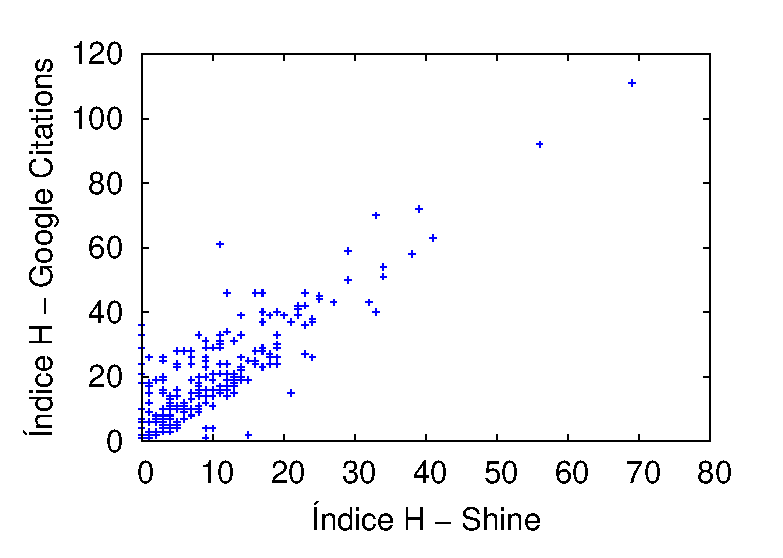
\includegraphics[scale=1]{../graficos/hindex/pt_BR/hindex_scatter_plot.eps}
\caption{Correlação entre o índice h estimado e o Google Citations}
\label{fig:hindex_scatter_plot}
\end{figure}
% \begin{figure}[!htb]
% \centering
% 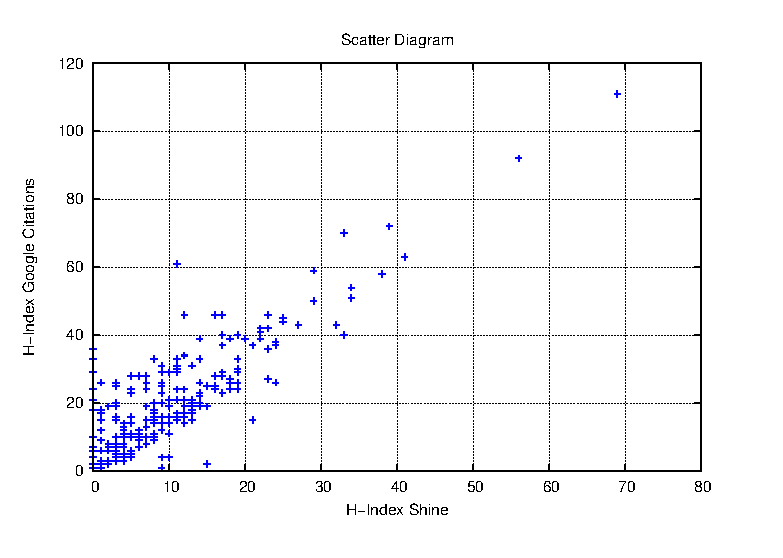
\includegraphics[scale=.5]{graficos/hindex/hindex_scatter_plot.eps}
% \caption{Correlation between the inferred h-index and Google Citations one}
% \vspace{-0.2cm}
% \label{fig:hindex_scatter_plot}
% \end{figure}
% 

% However, there is one important limitation with this strategy.  As SHINE does not track all the existent Computer Science conferences, researchers' h-index might be underestimated when computed
% with this data. To investigate this issue, we compared the h-index of a set of researchers with a profile on Google Scholar with their estimated h-index based on the SHINE data. For this, we
% randomly selected 10 researchers for each conference from Table~\ref{tab:sigs_conference_period} and extracted their h-indexes from their Google Scholar profiles.  In comparison
% with the h-index we estimated from SHINE, the Google Scholar values are, on average, 50\% higher. Figure~\ref{fig:hindex_scatter_plot} shows the scatter plot for the two h-index
% measures. We can note that although SHINE h-index is smaller, the two measures are highly correlated. The Pearson's correlation coefficient is 0.85, which indicates that researchers
% might have proportional h-index estimations in both systems. 

A segunda limitação está relacionada à evolução do índice~h ao longo do tempo. O 
SHINE coleta somente o total atual de citações de cada artigo, sendo possível estimar 
apenas o valor final do índice~h de um dado pesquisador. De forma análoga à abordagem 
anterior, selecionamos aleatoriamente 10 pesquisadores de cada conferência e extraímos 
do Google Citations o número de citações dos artigos de cada pesquisador ao longo 
do tempo, nos permitindo, assim, obter a curva de evolução do índice~h desses pesquisadores.

\cite{Acuna2012} apresentam um método que inclui equações capazes de predizer o índice~h 
de um pesquisador daqui a um, cinco ou dez anos. Desta forma, 
utilizamos cada equação para estimar o índice~h dos pesquisadores e comparamos com os 
dados coletados do Google Citations utilizando regressão linear, $R^2$. De acordo com 
a CDF (\textit{Cumulative Distribution Function}) na Figura~\ref{fig:calculos_nature}, 
podemos observar que a equação de um ano é a que mais se assemelha aos valores do Google
Citations, tendo mais de 70\% dos pesquisadores com $R^2$ superior a 60\%. Com base 
nas equações definidas por \cite{Acuna2012}, computamos o índice~h dos pesquisadores
utilizando três abordagens: (i) a primeira fixa o índice~h atual do pesquisador ao 
longo do tempo, (ii) em seguida utilizamos a equação capaz de prever o índice~h ano a ano 
dos pesquisadores definida por \cite{Acuna2012}, e (iii) por fim, utilizamos uma 
evolução linear do índice~h do pesquisador considerando a sua primeira e última data de publicação.
A Figura~\ref{fig:comprativo_evolucao_hindex} mostra a CDF da $R^2$ entre os valores 
do Google Scholar e os valores estimados utilizando as três abordagens propostas, sendo 
possível observar que a abordagem utilizando a evolução linear é a que mais se 
aproxima dos valores do Google Scholar, tendo mais de 60\% dos pesquisadores com $R^2$ superior a 80\%.

% \redcomment{Como base nos dados coletados, utilizamos três abordagens com o intuito de observar qual melhor representa a evolução do índice~h a partir do seu valor final. A primeira abordagem mantém 
% constante o índice~h final do pesquisador ao longo do tempo. Em seu trabalho, \cite{Acuna2012} apresentam três abordagens capazes de predizer o índice~h de um pesquisador, desta forma, 
% usamos cada método para estimar o índice~h dos pesquisadores, conforme apresentado na Figura~\ref{fig:calculos_nature}, sendo possível observar, de acordo com a CDF (\textit{Cumulative 
% Distribution Function}) da regressão linear, $R^2$, que a abordagem que prevê o índice~h ano a ano apresenta um melhor resultado, sendo esta apontada como a nossa segunda abordagem. 
% Por fim, a terceira e última abordagem consiste em utilizar uma evolução linear do índice~h do pesquisador considerando a sua primeira e última data de publicação. A 
% Figura~\ref{fig:comprativo_evolucao_hindex} mostra a CDF da $R^2$ entre os valores do Google Scholar e os valores estimados utilizando as três abordagens propostas, sendo 
% possível observar que a abordagem utilizando a evolução linear é a que mais se aproxima dos valores do Google Scholar, tendo mais de 60\% dos pesquisadores
% com valor superior a 80\% a $R^2$.}

\begin{figure}[!htb]
  \begin{center}
    \subfloat[Valores gerados utilizando o método proposto por \cite{Acuna2012}]{%
      \label{fig:calculos_nature}
      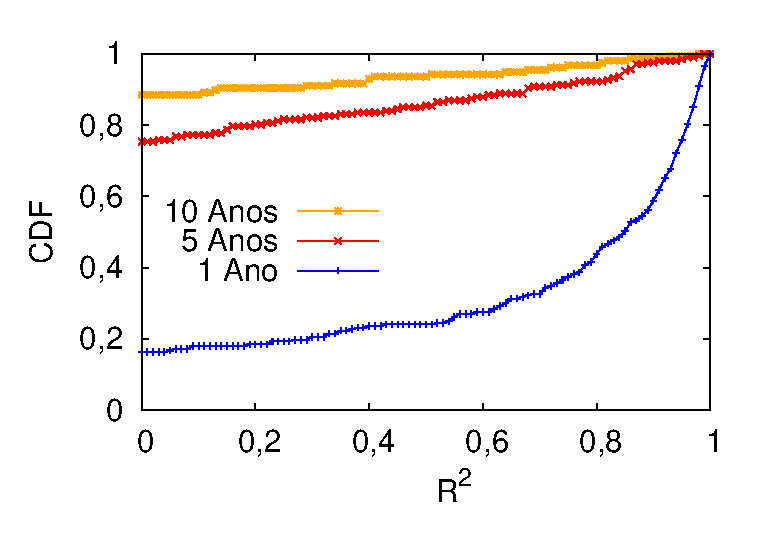
\includegraphics[scale=.5]{../graficos/hindex/pt_BR/nature_cdf.eps}
    }%
    \hspace{1cm}
    \subfloat[Valores gerados utilizando as três estratégias]{%
      \label{fig:comprativo_evolucao_hindex}
      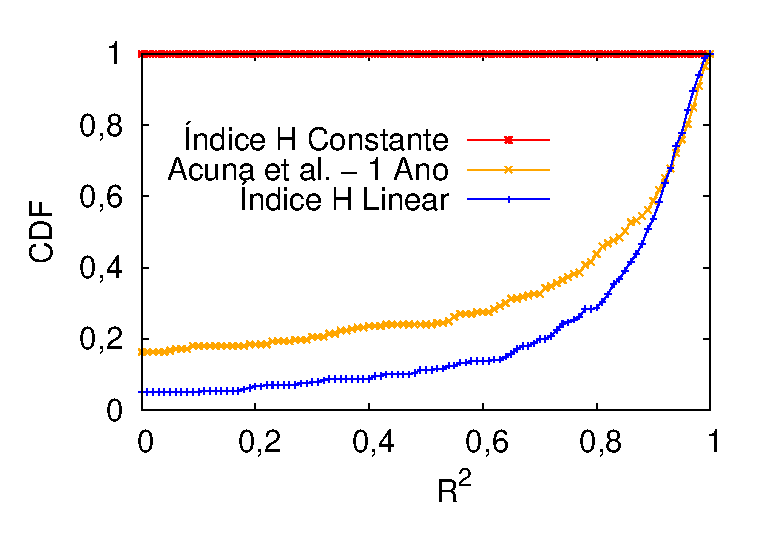
\includegraphics[scale=.5]{../graficos/hindex/pt_BR/linear_hindex_cdf.eps}
    }%
  \end{center}
  \caption{Evolução do índice~h}
  \label{fig:evolucao_hindex}
\end{figure}

%%%%%%%%%%%%%%%%%%%%%%%%%%%%%%%%%%%
\subsection{Definição dos Limiares}\label{sub:limiares}
%%%%%%%%%%%%%%%%%%%%%%%%%%%%%%%%%%%

Nossa estratégia para definir os dois limiares necessários para definir o núcleo das 
comunidades consiste em variar cada um deles e quantificar como eles impactam nas 
mudanças dos membros desse núcleo. Para medir essas mudanças, calculamos a
métrica \textit{resemblance}, conforme definida por~\cite{Viswanath2009}, que mede a 
fração dos membros do núcleo no tempo $t_0$ que permanecem no núcleo no tempo $t_1$.
Para cada comunidade, variamos o tamanho da janela de 1 a 5 anos e o tamanho do 
núcleo de 10\% a 60\% do total dos respectivos pesquisadores.
% Our strategy to define the two required thresholds consists of varying each of them and quantifying how they impact on the changes on the members of the community core. To measure these
% changes, we compute the resemblance metric, as used in~\cite{Viswanath:2009}, which measures the fraction of members in the core at time $t_0$ that remains in the core at time $t_1$. 
% For each community, we varied the window size from 1 to 5 years and the size of the community core from 10\% to 60\% of the entire community.
% % 
% % There are two important thresholds in our approach we need to define to determine the core of a scientific community.  The first is related to the time window in which the 
% % community core is computed. In other words, should we compute the community core at each year, at each two years, or for a larger time window? The second threshold is related to the
% % size of the community core. As we define the core of a community as the top researchers in terms of their core score during a certain time window, it is important to define the
% % threshold for choosing the top ones.

Intuitivamente, uma alta variação da métrica \textit{resemblance} indica uma escolha 
ruim dos limiares. Assim, procuramos por limiares cujas mudanças causassem pequenas 
alterações nos valores dessa métrica. A Figura~\ref{fig:averange_values_resemblance} 
mostra os valores do \textit{resemblance} em função do tamanho da janela, fornecendo 
diferentes curvas para o tamanho do núcleo da comunidade. Mostramos aqui apenas as 
curvas das comunidades SIGMOD e CHI, as curvas das demais comunidades podem ser encontradas 
no Apêndice~\ref{apendice:media_valores_resemblance}. Por inspeção visual definiríamos 
o tamanho do núcleo da comunidade como 10\% devido à proximidade das curvas e o tamanho 
da janela como 2 ou 3, uma vez que a maior parte das comunidades mostra um valor 
do \textit{resemblance} mais estável após esses valores. Para nos ajudar a decidir, calculamos 
o coeficiente angular das curvas com tamanho do núcleo de 10\% para cada comunidade e a 
média do coeficiente angular para elas. Com base nesses valores, definimos o tamanho da 
janela para nossos experimentos como sendo de 3 anos.
% Intuitively, high resemblance variations indicate bad threshold choices and, thus, we should seek for values in which threshold changes cause slight changes on resemblance.
% Figure~\ref{fig:averange_values_resemblance} shows the resemblance values as a function of the window size, providing different curves for the community core size.  We chose the
% SIGMOD and CHI communities for this analysis. The rest of the communities are omitted due to lack of space, but the same observations hold for them. By visual inspection we would set the core
% size as 10\% due to the proximity of the curves, and the window size as 2 or 3, as most of the communities showed a more stable resemblance after these values. To help us decide, we
% computed the angular coefficient for the 10\% core size curves of each community and obtained the average angular coefficient for them.  Based on this value, we chose the window
% size for our experiments as 3 years.

\begin{figure}[!htb]
  \begin{center}
    \subfloat[SIGMOD]{%
      \label{fig:sigmod_slide_window_top_list}
      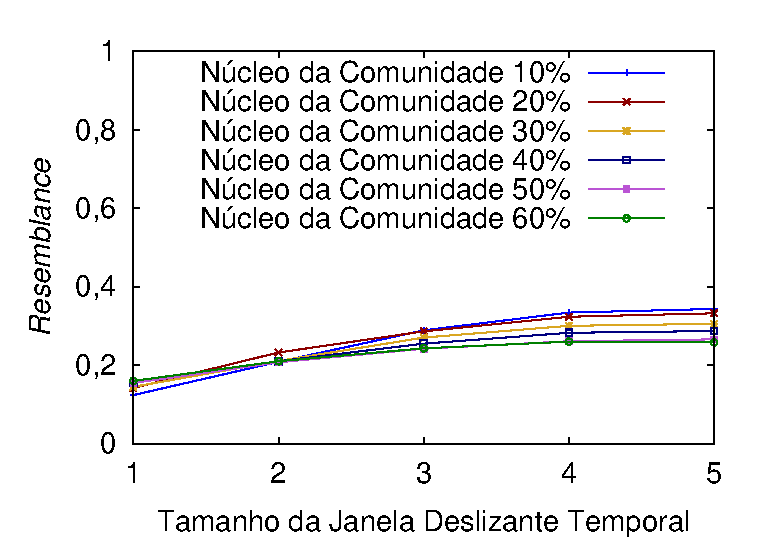
\includegraphics[scale=.6]{../graficos/window_core_size/pt_BR/sigmod_conference_arithmetic_slide_window_arithmetic_top_list.eps}
    }%
    \subfloat[CHI]{%
      \label{fig:chi_slide_window_top_list}
      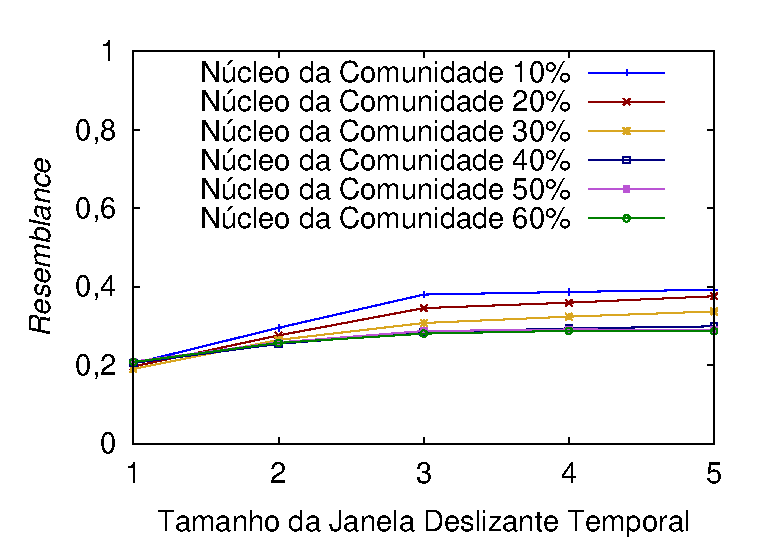
\includegraphics[scale=.6]{../graficos/window_core_size/pt_BR/chi_arithmetic_slide_window_arithmetic_top_list.eps}
    }%
  \end{center}
\caption{Média dos valores de \textit{resemblance}}
\label{fig:averange_values_resemblance}
\end{figure}
% \begin{figure}[!htb]
%   \begin{center}
%     \subfigure[SIGMOD]{%
%       \label{fig:sigmod_slide_window_top_list}
%       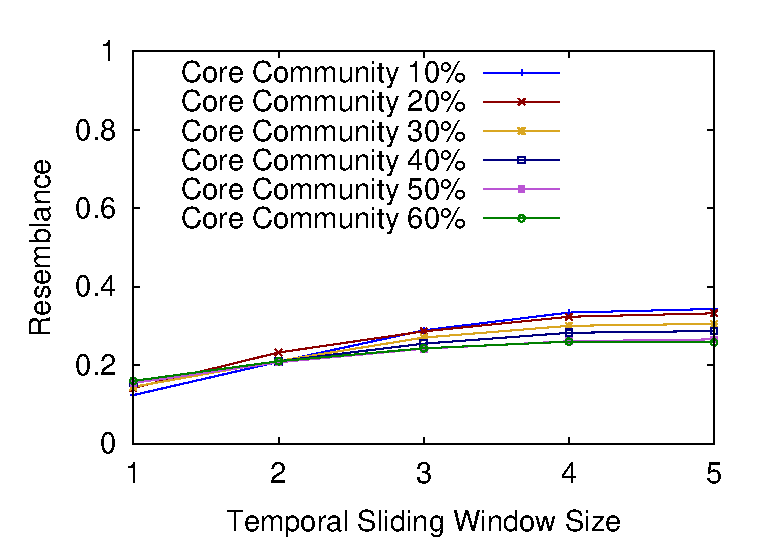
\includegraphics[scale=.33]{graficos/window_core_size/sigmod_slide_window_top_list.eps}
%     }%
%     \subfigure[CHI]{%
%       \label{fig:chi_slide_window_top_list}
%       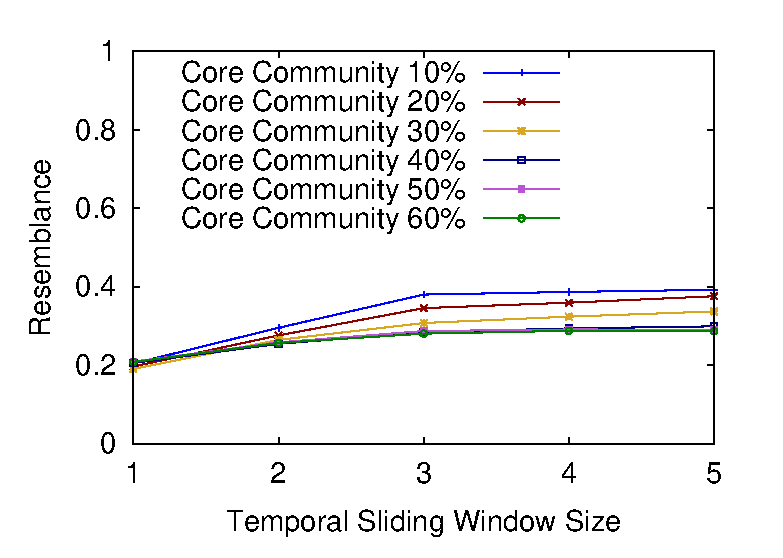
\includegraphics[scale=.33]{graficos/window_core_size/chi_slide_window_top_list.eps}
%     }%
%   \end{center}
% \vspace{-0.5cm}
% \caption{Average of the values of resemblance}
%  \label{fig:averange_values_resemblance}
% \end{figure}
% 

%%%%%%%%%%%%%%%%%%%%%%%%%%%%%%%%%%%
\subsection{Validação}
%%%%%%%%%%%%%%%%%%%%%%%%%%%%%%%%%%%

Com base no \textit{CoScore}, esperamos que os membros do núcleo da comunidade sejam pesquisadores que contribuam ativamente com publicações em uma determinada comunidade.
A validação desta suposição é, por natureza, subjetiva. Assim, fornecemos a seguir evidências que nossa abordagem captura corretamente essa característica esperada.
% Based on the core score value, we expect that the members of the community core would be standing researchers that actively contribute with publications to a certain community.
% The validation of this assumption is, by nature, subjective.  Thus, we provide next evidence that our approach correctly captures this expected characteristic.

\begin{figure}[!htb]
  \begin{center}
    \subfloat[Jon Kleinberg]{%
      \label{fig:cc_kleinberg}
      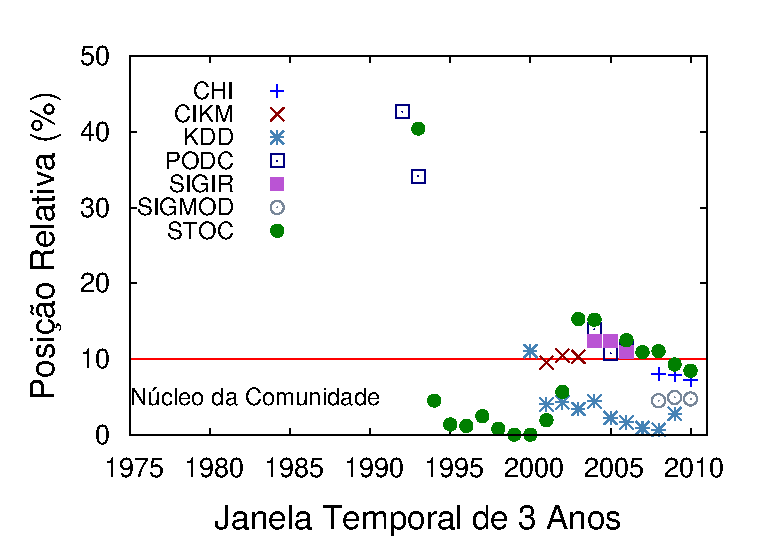
\includegraphics[scale=.6]{../graficos/validacao_core_community/pt_BR/cc_kleinberg_evolution.eps}
    }%
    \subfloat[Luis von Ahn]{%
      \label{fig:cc_luis_von_ahn}
      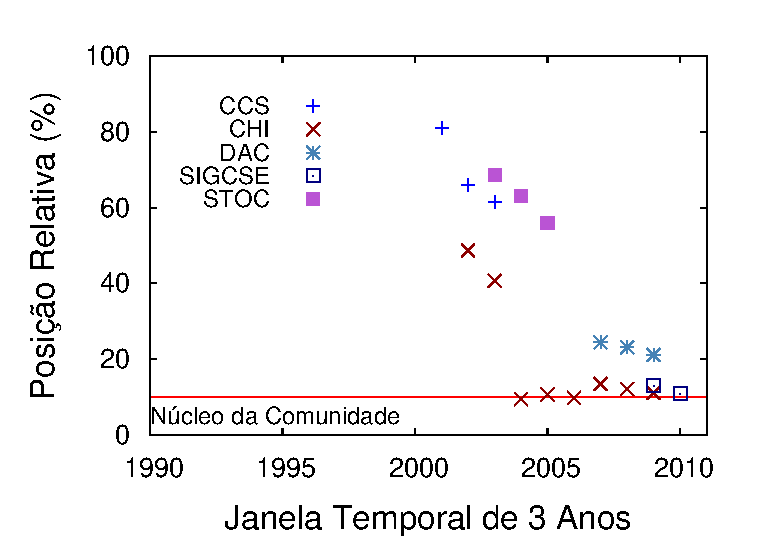
\includegraphics[scale=.6]{../graficos/validacao_core_community/pt_BR/cc_luis_von_ahn_evolution.eps}
    }%
  \end{center}
\caption{\textit{CoScore} de dois palestrantes convidados da WWW 2013}
 \label{fig:rank_core_score_authors}
\end{figure}

% \begin{figure}[!htb]
%   \begin{center}
%     \subfigure[Jon Kleinberg]{%
%       \label{fig:cc_kleinberg}
%       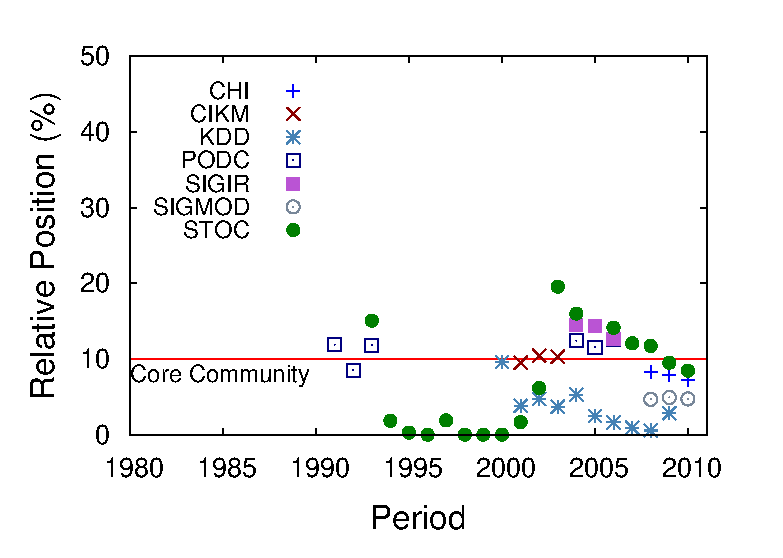
\includegraphics[scale=.33]{graficos/validacao_core_community/cc_kleinberg.eps}
%     }%
%     \subfigure[Luis von Ahn]{%
%       \label{fig:cc_luis_von_ahn}
%       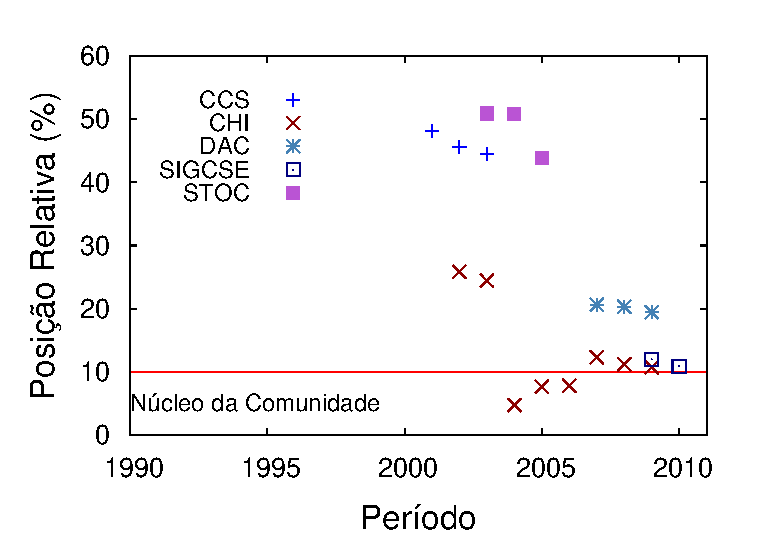
\includegraphics[scale=.33]{graficos/validacao_core_community/cc_luis_von_ahn.eps}
%     }%
%   \end{center}
% \vspace{-0.5cm}
% \caption{Core score of two WWW 2013 keynote speakers}
%  \label{fig:rank_core_score_authors}
% \end{figure}
% 

Primeiro, analisamos o \textit{CoScore} de dois palestrantes convidados da 
conferência WWW 2013 realizada recentemente no Rio de Janeiro: Jon Kleinberg 
e Luis von Ahn. A Figura~\ref{fig:rank_core_score_authors} mostra 
a posição em termos da percentagem (e.g., a posição 5\% de uma dada comunidade), 
desses dois pesquisadores nas comunidades em que eles têm publicado. A linha inferior 
divide os membros do núcleo da comunidade dos demais membros. Podemos notar que Jon 
Kleinberg foi membro do núcleo da comunidade STOC, uma conferência teórica, por anos. Mais 
precisamente, ele foi parte do núcleo da STOC por doze anos, publicando sete artigos 
na STOC em um único período de três anos. Com o envolvimento de Kleinberg na KDD, ele se tornou 
menos ativo na STOC e saiu do núcleo dessa comunidade por algum tempo. Durante esse 
período, ele publicou muitos artigos na KDD, enquanto suas publicações na STOC foram 
reduzindo. Com relação ao pesquisador Luis von Ahn, podemos notar que ele é mais ativo 
na comunidade CHI, na qual ele publicou seis artigos ao longo de sua vida acadêmica. Ele 
chegou ao núcleo da comunidade CHI em duas janelas de tempo, publicando quatro artigos 
na CHI em um único período.

% Primeiro, nós analisamos a pontuação do núcleo de dois palestrantes principais da WWW 2013: Jon Kleinberg e Luis von Ahn. A Figura~\ref{fig:rank_core_score_authors} mostra 
% a posição no ranking em termos da porcentagem (e.g., a posição 5\% de uma dada comunidade) destes dois pesquisadores nas comunidades que eles tenham publicado. A linha inferior 
% divide os membros do núcleo da comunidade dos demais membros. Nós podemos notar que Jon Kleinberg era um membro do núcleo da comunidade STOC, uma conferência teórica, por anos. Mais 
% precisamente, ele foi parte do núcleo da STOC por doze anos, publicando sete artigos na STOC em um único período de três anos. Com o envolvimento de Kleinberg na KDD, ele se tornou 
% menos ativo na STOC e saiu do núcleo dessa comunidade por algum tempo. Durante este período, ele publicou muitos artigos na KDD, enquanto suas publicações na STOC foram 
% reduzindo. Quando se trata de Luis von Ahn, nós podemos notar que ele é mais ativo na comunidade CHI, uma comunidade em que ele publicou seis artigos ao longo de sua vida 
% acadêmica. Ele chegou ao núcleo da comunidade CHI ao longo de três janelas de tempo consecutivas, publicando quatro artigos na CHI em um único período.

% First, we analyzed the core score of two WWW 2013 keynote speakers: Jon Kleinberg and Luis von Ahn.  Figure~\ref{fig:rank_core_score_authors} shows the ranking position in terms of
% percentage (e.g., position 5\% of that community) of these two researchers in the communities they have published. The bottom line divides the members of the community core from the others.
% We can note that Jon Kleinberg was a member of the community core of STOC, a theoretical conference, for years. More precisely, he was part of the STOC core for twelve years,
% publishing seven STOC papers in a single period of three years. With Kleinberg's involvement on KDD, he became less active in STOC and left the core of that community for some time.
% During this period, he published several KDD papers, while his STOC publications were reduced.  When it comes to Luis von Ahn, we can note that he is more active in
% the CHI community, a community in which he published six papers along his academic life. He reached the core of the CHI community along three consecutive time windows,
% publishing four CHI papers in a single period.


\begin{table*}[!hptb]
\centering
\caption{Pesquisadores das conferências CHI, ICSE, KDD e POPL que apareceram com mais 
frequência no núcleo da comunidade através dos anos.}
\label{tab:authors_frequency_core_community_grupo1}
{\fontsize{9.2}{11}\selectfont
\begin{tabular}{|c|c|c|c|} \hline
\textbf{CHI} & \textbf{ICSE} & \textbf{KDD} & \textbf{POPL}\\ \hline
\textbf{Scott E. Hudson} & \textbf{Victor R. Basili} & \textbf{Heikki Mannila} & Thomas W. Reps\\ \hline
\textbf{Hiroshi Ishii} & \textbf{Barry W. Boehm} & Hans-Peter Kriegel & Martín Abadi\\ \hline
\textbf{Steve Benford} & \textbf{Jeff Kramer} & \textbf{Jiawei Han} & John C. Mitchell\\ \hline
\textbf{George G. Robertson} & \textbf{Mary Shaw} & Martin Ester & Robert Harper\\ \hline
\textbf{Shumin Zhai} & Dewayne E. Perry & \textbf{Rakesh Agrawal} & Zohar Manna\\ \hline
\textbf{Brad A. Myers} & Don S. Batory & Bing Liu & Benjamin C. Pierce\\ \hline
\textbf{Robert E. Kraut} & Mary Jean Harrold & Ke Wang & Amir Pnueli$^\star$\\ \hline
\textbf{Elizabeth D. Mynatt} & \textbf{Lori A. Clarke} & \textbf{Padhraic Smyth} & \textbf{Barbara Liskov}$^\star$\\ \hline
\textbf{Ravin Balakrishnan} & Gruia-Catalin Roman & Philip S. Yu & Martin C. Rinard\\ \hline
\textbf{James A. Landay} & Premkumar T. Devanbu & Charu C. Aggarwal & Luca Cardelli\\ \hline
Ken Hinckley & Gail C. Murphy & \textbf{Vipin Kumar} & Thomas A. Henzinger\\ \hline
\textbf{Mary Czerwinski} & \textbf{Richard N. Taylor} & Wynne Hsu & \textbf{Ken Kennedy}\\ \hline
\textbf{Carl Gutwin} & \textbf{David Garlan} & Qiang Yang & \textbf{Matthias Felleisen}\\ \hline
\textbf{Gregory D. Abowd} & Michael D. Ernst & \textbf{Christos Faloutsos} & Edmund M. Clarke$^\star$\\ \hline
Michael J. Muller & James D. Herbsleb & William W. Cohen & Mitchell Wand\\ \hline
\textbf{Susan T. Dumais} & Lionel C. Briand & Pedro Domingos & David Walker\\ \hline
Loren G. Terveen & Gregg Rothermel & Eamonn J. Keogh & Simon L. Peyton Jones\\ \hline
\textbf{Steve Whittaker} & Kevin J. Sullivan & Alexander Tuzhilin & Shmuel Sagiv\\ \hline
W. Keith Edwards & \textbf{David Notkin} & Mohammed Javeed Zaki & Barbara G. Ryder\\ \hline
\textbf{John M. Carroll} & Douglas C. Schmidt & Mong-Li Lee & Alexander Aiken\\ \hline
\end{tabular}
% \par\medskip\footnotesize{$^\star$ Pesquisadores premiados por uma vida de inovação e liderança dentro daquela comunidade.}
% \par\medskip\footnotesize{$^\star$ Pesquisadores agraciados com \textit{A. M. Turing Award}.}
}
\end{table*}


\begin{table*}[!hptb]
\centering
\caption{Pesquisadores das conferências SIGCOMM, SIGGRAPH, SIGIR e SIGMOD que apareceram com mais 
frequência no núcleo da comunidade através dos anos.}
\label{tab:authors_frequency_core_community_grupo2}
{\fontsize{9.2}{11}\selectfont
\begin{tabular}{|c|c|c|c|} \hline
\textbf{SIGCOMM} & \textbf{SIGGRAPH} & \textbf{SIGIR} & \textbf{SIGMOD}\\ \hline
\textbf{Scott Shenker} & \textbf{Donald P. Greenberg} & \textbf{W. Bruce Croft} & \textbf{Michael Stonebraker}\\ \hline
George Varghese & \textbf{Pat Hanrahan} & Clement T. Yu & \textbf{David J. DeWitt}\\ \hline
\textbf{Donald F. Towsley} & Demetri Terzopoulos & \textbf{Gerard Salton} & \textbf{Philip A. Bernstein}\\ \hline
Ion Stoica & \textbf{David Salesin} & Alistair Moffat & H. V. Jagadish\\ \hline
Hui Zhang & \textbf{Michael F. Cohen} & \textbf{Susan T. Dumais} & Christos Faloutsos\\ \hline
Deborah Estrin & \textbf{Richard Szeliski} & James Allan & \textbf{Rakesh Agrawal}\\ \hline
Hari Balakrishnan & John F. Hughes & Yiming Yang & \textbf{Michael J. Carey}\\ \hline
Robert Morris & N. Magnenat-Thalmann & Edward A. Fox & \textbf{H. Garcia-Molina}\\ \hline
Thomas E. Anderson & \textbf{Tomoyuki Nishita} & James P. Callan & Jiawei Han\\ \hline
Ramesh Govindan & \textbf{Andrew P. Witkin} & Chris Buckley & Raghu Ramakrishnan\\ \hline
Srinivasan Seshan & Norman I. Badler & \textbf{C. J. van Rijsbergen} & Jeffrey F. Naughton\\ \hline
David Wetherall & \textbf{Peter Schröder} & Justin Zobel & \textbf{Jim Gray}$^\star$\\ \hline
Yin Zhang & Steven Feiner & Ellen M. Voorhees & Hans-Peter Kriegel\\ \hline
Jennifer Rexford & \textbf{Hugues Hoppe} & Mark Sanderson & Gerhard Weikum\\ \hline
Jia Wang & \textbf{Jessica K. Hodgins} & \textbf{Norbert Fuhr} & Philip S. Yu\\ \hline
J. J. Garcia-Luna-Aceves & \textbf{Greg Turk} & Nicholas J. Belkin & Divesh Srivastava\\ \hline
Randy H. Katz & \textbf{Marc Levoy} & Chengxiang Zhai & Joseph M. Hellerstein\\ \hline
Albert G. Greenberg & \textbf{P. Prusinkiewicz} & Charles L. A. Clarke & Krithi Ramamritham\\ \hline
Mark Handley & Eihachiro Nakamae & Alan F. Smeaton & Nick Roussopoulos\\ \hline
\textbf{Simon S. Lam} & Dimitris N. Metaxas & Gordon V. Cormack & \textbf{Surajit Chaudhuri}\\ \hline
\end{tabular}
% \par\medskip\footnotesize{$^\star$ Pesquisadores premiados por uma vida de inovação e liderança dentro daquela comunidade.}
% \par\medskip\footnotesize{$^\star$ Pesquisadores agraciados com \textit{A. M. Turing Award}.}
}
\end{table*}

% CHI
% 52 90 0.577777777778
% ICSE
% 15 23 0.652173913043
% KDD
% 9 12 0.75
% POPL
% 6 23 0.260869565217
% SIGCOMM
% 9 26 0.346153846154
% SIGGRAPH
% 21 42 0.5
% SIGIR
% 7 10 0.7
% SIGMOD
% 17 20 0.85

% \begin{table*}[!hptb]
% \centering
% \caption{Pesquisadores que apareceram com mais frequência no núcleo da comunidade através dos anos.}
% \label{tab:authors_frequency_core_community}
% {\fontsize{9.2}{11}\selectfont
% \begin{tabular}{|c|c|c|c|} \hline
% \textbf{KDD} & \textbf{SIGCOMM} & \textbf{SIGIR} & \textbf{SIGMOD}\\ \hline
% Heikki Mannila$^\star$ & Scott Shenker$^\star$ & W. Bruce Croft$^\star$ & David J. DeWitt$^\star$\\ \hline
% Jiawei Han$^\star$ & George Varghese & Clement T. Yu & Michael Stonebraker$^\star$\\ \hline
% Eamonn J. Keogh & Hui Zhang & Susan T. Dumais$^\star$ & H. V. Jagadish\\ \hline
% Martin Ester & Donald F. Towsley$^\star$ & James Allan & Rakesh Agrawal$^\star$\\ \hline
% Bing Liu & Hari Balakrishnan & Justin Zobel & Christos Faloutsos\\ \hline
% Padhraic Smyth$^\star$ & Ion Stoica & Alistair Moffat & Raghu Ramakrishnan\\ \hline
% Charu C. Aggarwal & Srinivasan Seshan & Norbert Fuhr$^\star$ & Jiawei Han\\ \hline
% Philip S. Yu & Deborah Estrin & James P. Callan & Gerhard Weikum\\ \hline
% Ke Wang & David Wetherall & Yiming Yang & Philip A. Bernstein$^\star$\\ \hline
% Hans-Peter Kriegel & Thomas E. Anderson & Edward A. Fox & Jeffrey F. Naughton\\ \hline
% Rakesh Agrawal$^\star$ & Jennifer Rexford & Gerard Salton$^\star$ & Hector Garcia-Molina$^\star$\\ \hline
% Jian Pei & Jia Wang & Ricardo A. Baeza-Yates & Michael J. Carey$^\star$\\ \hline
% Wynne Hsu & Ratul Mahajan & Jian-Yun Nie & Joseph M. Hellerstein\\ \hline
% Qiang Yang & Vern Paxson$^\star$ & Mark Sanderson & Philip S. Yu\\ \hline
% Christos Faloutsos$^\star$ & Mark Handley & Charles L. A. Clarke & Divesh Srivastava\\ \hline
% Huan Liu & Yin Zhang & Chris Buckley & Michael J. Franklin\\ \hline
% Mohammed Javeed Zaki & Peter Steenkiste & Chengxiang Zhai & Jennifer Widom$^\star$\\ \hline
% Pedro Domingos & Walter Willinger & Alan F. Smeaton & Hans-Peter Kriegel\\ \hline
% Jon M. Kleinberg & Ramesh Govindan & Zheng Chen & Hamid Pirahesh\\ \hline
% Vipin Kumar$^\star$ & Jon Crowcroft$^\star$ & Ophir Frieder & Surajit Chaudhuri$^\star$\\ \hline
% \end{tabular}
% \par\medskip\footnotesize{$^\star$ Pesquisadores premiados por uma vida de inovação e liderança dentro daquela comunidade.}
% }
% \end{table*}
% ----------------------
% \begin{table*}[!hptb]
% \centering
% \caption{Researchers who appear most often in the community core over the years}
% \label{tab:authors_frequency_core_community}
% {\small
% \begin{tabular}{|c|c|c|c|} \hline
% \bf{KDD} & \bf{SIGCOMM} & \bf{SIGIR} & \bf{SIGMOD}\\ \hline
% Heikki Mannila$^\star$ & Scott Shenker$^\star$ & W. Bruce Croft$^\star$ & David J. DeWitt$^\star$\\ \hline
% Jiawei Han$^\star$ & George Varghese & Clement T. Yu & Michael Stonebraker$^\star$\\ \hline
% Eamonn J. Keogh & Hui Zhang & Susan T. Dumais$^\star$ & H. V. Jagadish\\ \hline
% Martin Ester & Donald F. Towsley$^\star$ & James Allan & Rakesh Agrawal$^\star$\\ \hline
% Bing Liu & Hari Balakrishnan & Justin Zobel & Christos Faloutsos\\ \hline
% Padhraic Smyth$^\star$ & Ion Stoica & Alistair Moffat & Raghu Ramakrishnan\\ \hline
% Charu C. Aggarwal & Srinivasan Seshan & Norbert Fuhr$^\star$ & Jiawei Han\\ \hline
% Philip S. Yu & Deborah Estrin & James P. Callan & Gerhard Weikum\\ \hline
% Ke Wang & David Wetherall & Yiming Yang & Philip A. Bernstein$^\star$\\ \hline
% Hans-Peter Kriegel & Thomas E. Anderson & Edward A. Fox & Jeffrey F. Naughton\\ \hline
% Rakesh Agrawal$^\star$ & Jennifer Rexford & Gerard Salton$^\star$ & Hector Garcia-Molina$^\star$\\ \hline
% Jian Pei & Jia Wang & Ricardo A. Baeza-Yates & Michael J. Carey$^\star$\\ \hline
% Wynne Hsu & Ratul Mahajan & Jian-Yun Nie & Joseph M. Hellerstein\\ \hline
% Qiang Yang & Vern Paxson$^\star$ & Mark Sanderson & Philip S. Yu\\ \hline
% Christos Faloutsos$^\star$ & Mark Handley & Charles L. A. Clarke & Divesh Srivastava\\ \hline
% Huan Liu & Yin Zhang & Chris Buckley & Michael J. Franklin\\ \hline
% Mohammed Javeed Zaki & Peter Steenkiste & Chengxiang Zhai & Jennifer Widom$^\star$\\ \hline
% Pedro Domingos & Walter Willinger & Alan F. Smeaton & Hans-Peter Kriegel\\ \hline
% Jon M. Kleinberg & Ramesh Govindan & Zheng Chen & Hamid Pirahesh\\ \hline
% Vipin Kumar$^\star$ & Jon Crowcroft$^\star$ & Ophir Frieder & Surajit Chaudhuri$^\star$\\ \hline
% \end{tabular}
% \par\medskip\footnotesize{$^\star$ Researchers awarded by a lifetime of innovation and leadership inside that community.}
% }
% \vspace{-0.2cm}
% \end{table*}
% 

Em seguida, computamos a posição dos pesquisadores que aparecem com mais 
frequência no núcleo de suas comunidades científicas. Escolhemos 
as conferências CHI, ICSE, KDD, POPL, SIGCOMM, SIGIR e SIGMOD para 
mostrar os 20 pesquisadores melhores colocados, conforme destacado nas
Tabelas~\ref{tab:authors_frequency_core_community_grupo1}~e~\ref{tab:authors_frequency_core_community_grupo2}. 
Como podemos notar, vários pesquisadores renomados aparecem no topo dessas 
listas, incluindo os palestrantes convidados das últimas edições das respectivas 
conferências e pesquisadores premiados por suas contribuições naquelas comunidades, 
cujos nomes aparecem em negrito, incluindo alguns que também receberam o ACM \textit{A.M. 
Turing Award}\footnote{http://amturing.acm.org/byyear.cfm} (marcados com $^\star$). De fato, analisando os pesquisadores premiados 
de cada comunidade, descobrimos que grande parte deles apareceu no núcleo da 
comunidade pelo menos uma vez na história da conferência. Mais especificamente, estas 
frações são de 58\% dos membros premiados da CHI\footnote{http://www.sigchi.org/about/awards}, 
65\% para a ICSE\footnote{http://www.sigsoft.org/awards/outResAwd.htm}, 75\% para a 
KDD\footnote{http://www.sigkdd.org/awards\_innovation.php}, 26\% para a 
POPL\footnote{http://www.sigplan.org/Awards/Achievement/Main}, 35\% para a 
SIGCOMM\footnote{http://www.sigcomm.org/awards/sigcomm-awards}, 50\% para a 
SIGGRAPH\footnote{http://www.siggraph.org/participate/awards}, 70\% para a
SIGIR\footnote{http://www.sigir.org/awards/awards.html}, e 85\% para a 
SIGMOD\footnote{http://www.sigmod.org/sigmod-awards}. Exceto para as conferências SIGCOMM 
e POPL (SIGPLAN), cujos SIGs patrocinam outros eventos que não foram considerados 
em nosso conjunto de dados, as outras seis comunidades apresentam um número muito 
alto de membros premiados que aparecem pelo menos uma vez em seus respectivos 
núcleos. Além disso, podemos observar que a comunidade POPL possui pelo menos três 
pesquisadores que receberam o ACM \textit{A.M. Turing Award}, 
um dos mais importantes prêmios da comunidade científica. Estas observações fornecem evidências 
que nossa abordagem captura corretamente a noção do núcleo de uma comunidade científica.

% Em seguida, nós calculamos o ranking dos pesquisadores que aparecem com mais frequência no núcleo da comunidade de cada comunidade científica. Nós escolhemos 
% as conferências KDD, SIGCOMM, SIGIR e SIGMOD para mostrar seus 20 pesquisadores melhores colocados, conforme apresentado na Tabela~\ref{tab:authors_frequency_core_community}. Como 
% podemos notar, vários grandes nomes aparecem no topo da lista, incluindo os principais palestrantes das últimas edições destas comunidades, bem como pesquisadores 
% premiados por seu tempo de vida de constribuições naquela comunidades. De fato, analizando os pesquisadores premiados de cada comunidade, nós descobrimos que
% grande parte deles apareceram no núcleo da comunidade pelo menos uma vez na história da conferênica. Mais especificamente, estas frações são de 75\% dos membros premiados 
% da KDD\footnote{http://www.sigkdd.org/awards\_innovation.php}, 35\% para a SIGCOMM\footnote{http://www.sigcomm.org/awards/sigcomm-awards}, 60\% para a
% SIGIR\footnote{http://www.sigir.org/awards/awards.html}, e 80\% para a SIGMOD\footnote{http://www.sigmod.org/sigmod-awards}. Exceto para a SIGCOMM, uma comunidade 
% com muitos eventos patrocinados que não foram considerados em nosso conjunto de dados, as outras três comunidades apresentam um número muito alto de membros premiados 
% que aparecem pelo menos uma vez no núcleo da comunidade. Estas observações fornecem evidências que nossa abordagem captura corretamente a noção de um núcleo em comunidades científicas.

% Then, we computed a ranking of researchers that appear most often in the community core of each scientific community. We chose the KDD, SIGCOMM, SIGIR, and SIGMOD communities to
% show their top 20 researchers in Table~\ref{tab:authors_frequency_core_community}.  As we can note, several big names appear in this top list, including past keynote speakers of
% these conferences as well as awarded researchers by their life time contributions in that community. Indeed, by analyzing the awarded researchers from each community we found that
% a large fraction of them appeared in the community core at least one time in the conference history. More specifically, these fractions are 75\% of the awarded
% KDD\footnote{http://www.sigkdd.org/awards\_innovation.php} members, 35\% for SIGCOMM\footnote{http://www.sigcomm.org/awards/sigcomm-awards}, 60\% for
% SIGIR\footnote{http://www.sigir.org/awards/awards.html}, and 80\% for SIGMOD\footnote{http://www.sigmod.org/sigmod-awards}.  Except for SIGCOMM, a community with many sponsored
% events that were not considered in our datasets, the other three communities presented very high numbers of awarded members that appear at least one time in the community core. These
% observations provide evidence that our approach correctly captures the notion of a scientific community core.